\documentclass[aps,prl,twocolumn, superscriptaddress,nobalancelastpage]{revtex4}
\usepackage{graphicx}
\usepackage{amssymb}
\usepackage{amsmath}
\usepackage{color}
\usepackage{academicons}
\usepackage{xcolor}



\begin{document}


\title{Subwavelength grating optical ring resonator devices for biosensing applications} 



\author{Daniel Hutama}
\author{Sam Lantela}
\author{Yeseul Lee}
\affiliation{Dept. of Electrical \& Computer Engineering, McGill University, Montr\'eal, Qu\'ebec, H3A 0E9, Canada}

\date{\today}
\begin{abstract}
\noindent \textbf{Abstract:}  One notable development in optical mircroring biosensors is the use of subwavelength grating (SWG) waveguides due to their increased sensitivity to index changes in the waveguide cladding material.  Ring devices based on SWG waveguides have substantial commercial potential due to their wide range of applications and compatibility with mainstream CMOS foundry processes.  Although such biosensors continue to see high levels of academic research activity, they have yet to make a large-scale breakthrough in commercialized frontline medical diagnostics equipment.  After presenting the operational principles of SWG ring biosensors and discussing the state-of-the-art in SWG ring-based biosensing, we analyze the challenges faced by silicon photonics biosensing technology. In particular, we examine the difficulties faced in commercializing silicon photonic biosensing devices and compare their performance with conventional biosensing assays. 
\end{abstract}
\pacs{}
\maketitle

\section{I. Introduction}
\vspace{-1em}

Silicon photonic biosensors based on the optical ring resonator (ORR) rely on the interaction of an evanescent electromagnetic field with the waveguide's surrounding cladding material. Such biosensors are able to detect analytes in real-time and without prior target labeling. In addition, the ability to fabricate multiple devices on a single chip using existing CMOS foundry processes allows for the possibility of performing several tests in parallel with a single biological sample. Recent developments in ORR biosensing devices have brought subwavelength grating (SWG) ring structures to the forefront of the emerging technology \cite{swg1, swg2, labelfree}.

Our goal is to present theoretical insight into the operational principles of SWG ORR biosensing devices, as well as to explore their practical limitations in comparison to contemporary frontline medical diagnostic biosensing devices. This paper is structured as follows: First, we briefly describe the operation of one of the most popular biosensing devices used in frontline medical diagnostics. We then present the theory behind subwavelength grating waveguides. After describing the operation of SWG waveguides, we discuss ring resonator devices and describe important parameters for the application of silicon photonic biosensing. Following this, we present an evaluation of SWG ORR biosensing devices in comparison with conventional biosensors.

\vspace{-1em}
\section{II. Conventional Biosensor Assays}
\vspace{-1em}

In this section, we briefly describe the operation of conventional biosensor assays used in frontline medical diagnostics. Conventional assays often require the use of a label, which is required to detect the analyte of interest. One of the most popular labels used in immunoassays are enzymes. Such immunoassays utilizing enzymes are referred to as enzyme-linked immunosorbent assays (ELISAs). Common enzymes used include alkaline phosphatase (ALP) and horseradish peroxidase (HRP), as these enzymes produce color changes upon interaction with particular reagents. For instance, common reagents include \textit{p}-nitrophenyl phosphate (PNPP), which turns yellow in the presence of ALP, and \textit{o}-phenylenediamine dihydrochloride (OPD),  which turns amber upon catalysis with HRP \cite{thermofisher}. 

There are several types of ELISA tests, with the most popular type being the indirect ELISA. A typical ELISA apparatus consists of a plate with 96 wells, in which serially diluted samples are placed and tested. The steps of the indirect ELISA are as follows: First, the bottoms of wells in an ELISA plate are coated with an antigen of interest, as shown in the top left of FIG. \ref{fig:ELISA_well}. A blocking agent, such as bovine serum albumin, is added to prevent non-specific binding to antigens in the well. Second, the patient's serum containing the target antibodies (analytes) is added to the ELISA well, as shown in the top right of FIG. \ref{fig:ELISA_well}. Wells are then washed out to remove any unbound antibodies. Third, a solution containing secondary animal antibodies against human antibodies is added to the well. These animal antibodies, shown in the bottom left of FIG. \ref{fig:ELISA_well}, are covalently conjugated to an enzyme, which acts as the test's label. The well is again washed out to remove any unbound enzyme conjugated antibodies. Finally, a colorigenic enzyme substrate (reagent), shown in the bottom right of FIG. \ref{fig:ELISA_well}, is added to the well. The substrate interacts with the conjugated enzyme to produce a visible color change. The concentration of analyte present can be calculated via spectrophotometric methods, or by observing the number of serially diluted wells that yield a positive reading.

Although ELISA is highly sensitive, with detection limits as low as around 1 picomole, the process is quite lengthy, requiring analysis times of about 1 hour \cite{mechbiosensors}. In addition, the requirement for specialized labels and reagents used in indirect ELISA not only adds to the process's cost, but also required labor time, and thus the patient's time-to-diagnosis. As we will discuss in following sections, the need for both the label and the corresponding reagent can be eliminated when designing a silicon photonic biosensor \cite{labelfree}.

\pagebreak

 \begin{figure}[!h]
    \centering
    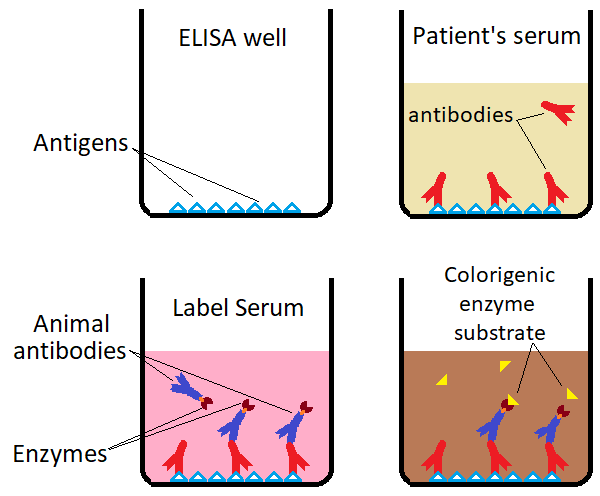
\includegraphics[width=7cm]{ELISA_well.png}
    \caption{Operational steps of a conventional enzyme-linked immunosorbent assay (ELISA). In the top left, the walls of the ELISA well are incubated with antigens. The top right shows the target antibodies in the patient's serum binding to the antigens in the well. The well is then washed to remove unbound antibodies. In the subsequent step, the label serum containing enzyme-linked secondary antibodies is added. The secondary antibodies bind to the primary antibodies and the well is washed again to remove unbound secondary antibodies. Finally, the reagent is added to elicit a color change upon catalysis with the enzyme.}
    \label{fig:ELISA_well}
\end{figure}

In order to be useful as a biosensor, a silicon photonic waveguide must first be functionalized by coating its surface with receptor biomolecules \cite{swg1}. As in ELISA, these receptors must bind, with a high degree of specificity, to the analyte. For instance, a biosensor might be based on an antibody-antigen pairs, in which antibodies will only attach to their corresponding antigens. When a sample containing the analyte is placed in contact with the waveguide, the analyte binds to the surface receptors, causing a change to the local index. The presence of analytes is then inferred by the corresponding change in output signal. Thus, the \textit{specificity} of photonic biosensors depends on the choice of surface rececptors, while the device's \textit{sensitivity} depends on the geometric implementation of the photonic waveguides. We will focus on the latter, particularly on how SWG ORRs are able to achieve much higher sensitivities than other designs.

\vspace{-1em}
\section{III. Subwavelength grating waveguides}
\vspace{-1em}

While conventional strip waveguides consist of a high refractive index core, SWG waveguides consist of an alternating arrangement of high-refractive index and low-refractive index segments \cite{OGswg}. FIG. \ref{fig:SWGdiagram} illustrates an SWG waveguide formed by a periodic arrangement of high-refractive index Si embedded on low-refractive index SiO$_2$ substrate. The SWG is characterized by a height $H$, width $W$, grating period $\Lambda$, and duty cycle $DC= L_\text{Si}/\Lambda$, where $L_\text{Si}$ is the length of the high-refractive index material (silicon) measured in the direction of propagation. 

\begin{figure}[!ht]
    \centering
    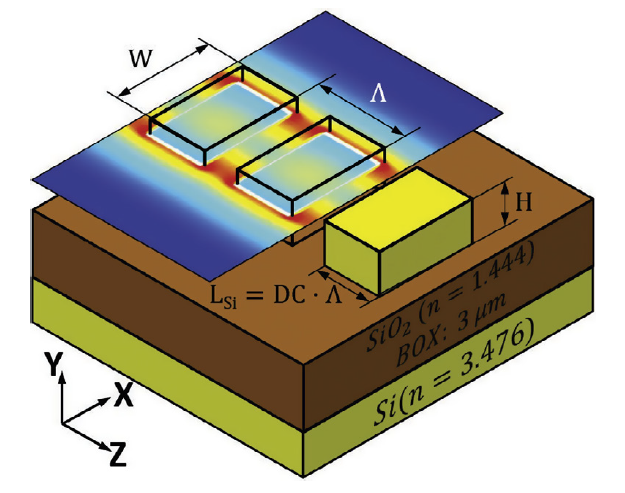
\includegraphics[width=6cm]{swgwaveguide2.png}
    \caption{From \cite{swg1}. Schematic of an SWG waveguide with constant pitch $\Lambda$ and duty cycle $DC = L_\text{Si}/\Lambda$. The electric field profile in the $xz$ plane is shown at $y = H/2$.}
    \label{fig:SWGdiagram}
\end{figure}

Electromagnetic fields in periodic grating waveguides excite Bloch-Floquet modes \cite{PhotonicCrystalsText}. These Bloch-Floquet modes are the natural modes of periodic media, and have mechanics that can be treated analogously to electron wavefunctions in a periodic crystal structure. In particular, the electric field of a Bloch-Floquet mode propagating through a uniform period waveguide in the $\hat{z}$ direction can be described by $E(x,y,z+\Lambda) = E_B(x,y,z)e^{-\gamma_B\Lambda}$, where $E_B(x,y,z)$ is the Bloch mode field distribution within a single period $\Lambda$, and $\gamma_B$ is the associated complex propagation constant. In general, $\gamma_B = \alpha_B + jk_B$, and $k_B = (2\pi/\lambda)n_B$, where $\alpha_B$ is the attenuation constant, $k_B$ is the propagation constant, and $n_B$ is the effective index of the Bloch-Floquet mode \cite{HalirReview}. 


For a given grating pitch $\Lambda$, the behavior of a periodic waveguide depends strongly on the free-space wavelength $\lambda$. In particular, depending on $\overline{\lambda} = \lambda/\Lambda$ (i.e. the ratio of free-space wavelength to grating pitch), the waveguide can operate in one of three regimes: (i) diffraction, in which the waveguide segments scatter an incoming beam away from the waveguide; (ii) reflection, in which an input beam from a conventional strip waveguide is reflected back into the input and gradually attenuated in the periodic waveguide; (iii) subwavelength, in which diffraction and reflection effects are suppressed \cite{HalirReview}. 

 \begin{figure}[!h]
    \centering
    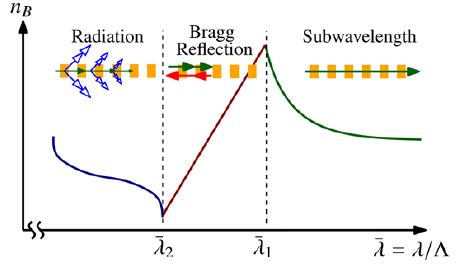
\includegraphics[width=7cm]{swgoperation.png}
    \caption{From \cite{HalirReview}. Bloch-Floquet mode effective index ($n_B$) as a function of the wavelength-to-pitch ratio $\overline{\lambda} = \lambda/\Lambda$.}
    \label{fig:SWGoperation}
\end{figure}

\pagebreak

\onecolumngrid

 \begin{figure}[!ht]
    \centering
    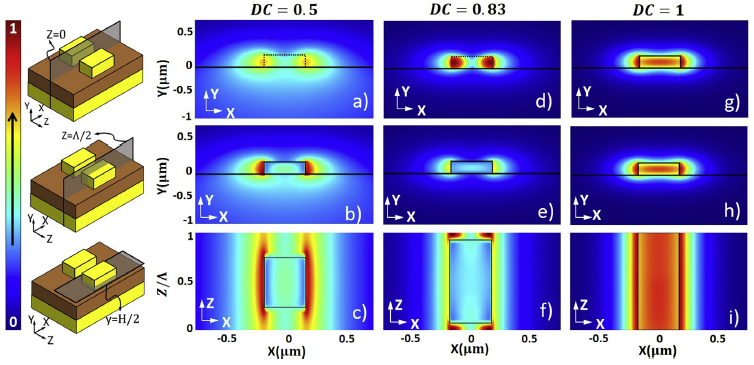
\includegraphics[width=15cm]{swgfield.png}
    \caption{From \cite{swg1}. Electric field distribution for various duty cycles with $W=350$ nm, $H=220$ nm, and $\Lambda = 250$ nm. The case of $DC=1$ corresponds to a conventional strip waveguide.}
    \label{fig:swgfield}
\end{figure}

\twocolumngrid

As shown in FIG. \ref{fig:SWGoperation}, light is radiated away from the waveguide for wavelengths comparable to the pitch of the grating (i.e. $\lambda/\Lambda <\overline{\lambda}_1$). Within the bandgap ($\overline{\lambda}_1<\overline{\lambda}<\overline{\lambda}_2$), the effective index follows the linear relation $n_B^{\text{Bragg}} \sim \frac{1}{2}\overline{\lambda}$. The subwavelength operating regime is reached when $n_B$ drops below the Bragg condition such that $n_B<n_B^{\text{Bragg}}$ \cite{HalirReview}. In this regime, diffraction and reflection effects are suppressed, and the SWG structure admits light as if it were a homogeneous waveguide. While conventional strip waveguides have strong optical confinement due high cladding-core index contrast, SWG waveguides have more field delocalization, with a greater proportion of the propagating signal residing outside of the core waveguide material. More precisely, the field profile reaches further into the waveguide's cladding region as shown in FIG. \ref{fig:swgfield}. For the application of biosensing, this translates to a higher modal field overlap with the analyte, resulting in increased sensitivity \cite{EvFieldBio}.

\section{IV. Optical Ring Resonators and sensor performance metrics}
\vspace{-1em}

An optical ring resonator (ORR) is said to be ``on resonance'' when the propagating wavelength fits an integer number of times inside the optical length of the ring cavity \cite{sipORRs}. In other words, 
\begin{equation}
    \lambda_\text{res} = \frac{2\pi r n_\text{eff}}{m}, \qquad m \in \mathbb{Z}^+,
    \label{eq:lamdares}
\end{equation}
where $r$ is the radius of the ring and $n_\text{eff}$ is the effective index of the guided mode. When an input waveguide is placed in close proximity to an ORR, the incoming signal will selectively couple from the waveguide to the resonator, depending on if the wavelength of the signal satisfies the resonance condition of the ORR.

Molecular binding occurs when analytes come into contact with a functionalized surface. The adsorption of analytes to the surface of a functionalized ORR causes a change in the local effective index, thus inducing a change in the ORR's resonant wavelength, as evident from equation \eqref{eq:lamdares}. By examining the shift in $\lambda_\text{res}$, we can determine the concentration of a given analyte in the sample. In order to do this, we must first define several metrics. The most important metrics for quantifying ORR sensor performance are as follows: (1) Sensitivity ($S$), (2) Resonator Quality Factor ($Q$), and (3) the Limit of Detection (LoD) \cite{sipresonators}. This remainder of this section is concerned with the description of each of these metrics.

\vspace{-1em}
\subsection{1. Sensitivity ($S$)}
\vspace{-1em}

We can quantitatively define sensitivity as having two components, $S= S_aS_w$. The first component, $S_a$ is attributed to the architecture of the sensing device, while the second component, $S_w$, is attributed to the waveguide mode sensitivity. For ring resonators, the architecture sensitivity is given by $S_a = \frac{\lambda_\text{res}}{n_g}$ \cite{swg1}, where $n_g$ is the group index, which can be obtained from the ring's free spectral range ($FSR$) by: $n_g = \frac{\lambda_\text{res}^2}{2\pi r \cdot FSR}$ \cite{swg3}.

The waveguide sensitivity parameter $S_w$ serves to map the process of molecular binding to variations in the effective index, $n_\text{eff}$. In particular we define:
\begin{equation}
    S_w = \frac{\partial n_\text{eff}}{\partial \Gamma},
    \label{eq:Sw}
\end{equation}
where $\partial \Gamma$ is the variation of a physical parameter of interest \cite{sipresonators}. Typically, $\Gamma$ either refers to the refractive index of the cladding, $n_c$, or the thickness of the adsorbed biomolecular layer, $t_\text{ad}$.

The case in which $\partial \Gamma = \partial n_c$ in equation \eqref{eq:Sw}, is referred to as the waveguide bulk sensitivity, $S_{w,b} = \frac{\partial n_\text{eff}}{\partial n_c}$. The total bulk sensitivity, being the change in resonant wavelength ($\Delta \lambda_\text{res}$) per unit change in refractive index of the cladding ($\Delta n_\text{clad}$), can then be expressed as follows \cite{swg3}:
\begin{equation}
    S_b = \frac{\Delta \lambda_\text{res}}{\Delta n_\text{clad}} = \frac{\lambda_\text{res}}{n_g}\left(\frac{\partial n_\text{eff}}{\partial n_\text{clad}}\right) \qquad \left[\frac{\text{nm}}{\text{RIU}}\right].
    \label{eq:Sbulk}
\end{equation}
Alternatively, the case in which $\partial \Gamma = \partial t_\text{ad}$ is referred to as the waveguide surface sensitivity,  $S_{w,s} = \frac{\partial n_\text{eff}}{\partial t_\text{ad}}$. The total surface sensitivity, being the change in the resonant wavelength ($\Delta \lambda_\text{res}$) per unit change in the thickness of the adsorbed biomolecular layer ($ \Delta t_\text{ad}$), can then be expressed as follows:
\begin{equation}
    S_s = \frac{\Delta \lambda_\text{res}}{\Delta t_\text{ad}} = \frac{\lambda_\text{res}}{n_g}\left(\frac{\partial n_\text{eff}}{\partial t_\text{ad}}\right) \qquad \left[\frac{\text{nm}}{\text{nm}}\right].
    \label{eq:Ssurf}
\end{equation}
While these electromagnetic definitions of sensitivity are useful to a photonic systems designer, they can also be made useful from a biochemical perspective \cite{swg1}. In particular, we can map the waveguide bulk sensitivity as $S_{w,b} \to \frac{\partial n_\text{eff}}{\partial c}$, where $\partial c$ is the variation in molar concentration with units of moles per liter $\left[M\right]$. This results in a total bulk sensitivity with units of $\left[\frac{\text{nm}}{M}\right]$, interpreted as the resonant wavelength shift per unit change in molarity. Similarly, we can map the waveguide surface sensitivity can as $S_{w,s} \to \frac{\partial n_\text{eff}}{\partial \rho_s}$, where $\partial \rho_s$ is the variation in mass surface density of the adsorbed layer with units of $\left[\frac{\text{pg}}{\text{mm}^2}\right]$. This results in a total surface sensitivity with units of $\left[\frac{\text{nm}}{\text{pg}/\text{mm}^2}\right]$, interpreted as the resonant wavelength shift per unit change in adsorbed layer mass surface density.
\vspace{-1em}
\subsection{2. Resonator Quality Factor ($Q$)}
\vspace{-1em}
The resonator quality factor $Q$ is a measure of the sharpness of resonances in the optical transmission spectrum. In particular, $Q = \frac{\lambda_\text{res}}{\Delta \lambda_{3\text{dB}}}$, where $\Delta \lambda_{3\text{dB}}$ is the resonance 3 dB linewidth. 

The $Q$ factor is physically related to the optical confinement factor and the amount of energy lost per cycle. Since conventional strip waveguides have higher confinement factors and lower propagation losses compared with SWG waveguides, they are more efficient in terms of power. These effects translate to conventional strip ORRs having higher $Q$-factors, meaning that the light circulates longer and interacts with the analyte over a greater number of circulations. However, since most of the energy travels inside the waveguide structure due to the high optical confinement, conventional strip ORRs are less sensitive to a changes in cladding refractive index. Thus, although conventional ORRs tend to have higher $Q$-factors, they tend to have lower bulk and surface sensitivities. 

\vspace{-1em}
\subsection{3. Limit of Detection (LoD)}
\vspace{-1em}

The significance of the trade-off between sensitivity, $S$, and quality factor, $Q$, becomes apparent when considering the biosensor's limit of detection (LoD), which is the minimum amount of detectable variation in the physical parameter $\Gamma$ from equation \eqref{eq:Sw}. For a variation $\partial \Gamma$ that causes the minimum detectable resonance shift $\Delta \lambda_\text{min}$, the LoD is given by $\text{LoD} = \frac{\Delta \lambda_\text{min}}{S}$, where $S$ can refer to either bulk sensitivity $S_b$ or surface sensitivity $S_s$. When comparing the performance of different \textit{resonant} sensors, a more useful metric is the intrisic limit of detection (iLoD), which is defined by setting the system resolution to the resonance 3 dB linewidth $\Delta \lambda_\text{3dB}$. In other words, \begin{equation}
\text{iLoD} = \frac{\Delta\lambda_\text{3dB}}{S} = \frac{\lambda_\text{res}}{Q\cdot S}.
\label{eq:iLoD}
\end{equation}
Thus, the iLoD of equation \eqref{eq:iLoD} provides a means for quantitatively comparing the performance of strip ORRs and SWG ORRs, even while considering the trade-offs between sensitivity and $Q$-factor. 

\section{V. SWG Optical Ring Resonators} %SWGMR -> SWG ORR for consistency
\vspace{-1em}
% will merge this info into previous section and focus on SWG ORRs here
%In the case of optical ring resonators there is a restriction on the wavelengths which can form modes on the waveguide. This restriction is based on the discrete solutions to Maxwell's equations and can be expressed as the phase condition: the phase shift after one cycle through the ring must be a multiple of 2$\pi$. As the cladding index changes due to analyte being deposited on the waveguide's surface there is a shift in the resonant wavelength of the ring resonator. This is caused by the slight variation of the boundary condition between the core and cladding resulting in a changing critical angle, thus changing the fundamental mode and resonant wavelength. The quality factor is of significant interest in ring resonator structures since it determines the ratio of energy stored by the structure to the energy lost per cycle, as such the quality factor is significantly related to the confinement factor. Since optical ring resonators have relatively high confinement factors they are efficient in terms of power. The advantages of conventional optical ring resonators is their simplicity and high quality factors however the disadvantage is that, since most of the energy travels inside the waveguide structure (high confinement), they are less sensitive to a change in refractive index in the cladding material. Thus optical ring resonators will have lower bulk and surface sensitivities. 
In this section, we evaluate the performance of SWG ORRs and compare with conventional ORRs for biosensing applications.

In the case of SWG ORRs the analytical approach is that of the effective refractive index method. As discussed in the section on SWG waveguides, there are 3 regimes of operation for Bragg gratings (radiation, reflection and subwavelength), for our purposes we are interested in the subwavelength case. In this regime, waveguide behaves if it were a continuous waveguide with reduced refractive index ($n_\text{core-eq}$). In particular, we have
\begin{equation}
    n_\text{core-eq} = n_\text{clad} + \eta \Delta n,
    \label{eq:n_eq}
\end{equation}
where $\eta$ is the duty cycle, and $\Delta n$ is the refractive index contrast:  $\Delta n = n_\text{core} - n_\text{clad}$ \cite{swg3}. Using this method, we can greatly simplify analysis of SWG ORRs, treating them as composed of conventional waveguides with reduced index contrast. The reduced index contrast results in one the the primary advantages; that is, most of the energy is carried outside the the core material. As a result,SWG ORRs have much greater sensitivities to changing refractive indices in the cladding material. 

While all ORRs experience bend losses, losses with SWG ORRs is noticeably higher, resulting in lower $Q$-factors. 

One limitation of conventional SWG ORR is the size. A large bend loss occurs in small radius of SWG ORR. With the trapezoidal silicon pillars (T-SWG ORR), we can significantly reduce the bend loss and manufacture the small radius SWG ORR. The schematic of 5um radius T-SWG ORR is in FIG.5.
%% micrometer in latex
With the time-domain coupled-mode theory, the quality factor $Q$ can be calculated with
\begin{equation}
    \frac{1}{Q} = \frac{1}{Q_C}+\frac{1}{Q_0}
\end{equation}
where $Q_0$ is the intrinsic quality factor and $Q_C$ is the coupling quality factor which depends on the coupling strength between SWG ORR and the bus waveguide. To increase the quality factor of the SWG ORR, it is necessary to increase not only the coupling quality factor by increasing the gap between SWG ORR and buss waveguide, but also the intrinsic quality factor. The large bend loss is the main factor which limits $Q_0$. Therfore, it is important to minimize bend loss in small radius SWG ORR. 


%% conventional stripWGORR 
%% hard to have high quality factor why? 1) high Q factor requires high light confinement for low loss 2) high light confinement -> limited light matter interaction






\pagebreak
% this needs to be at the top a page in the final version
\onecolumngrid

 \begin{figure}[!ht]
    \centering
    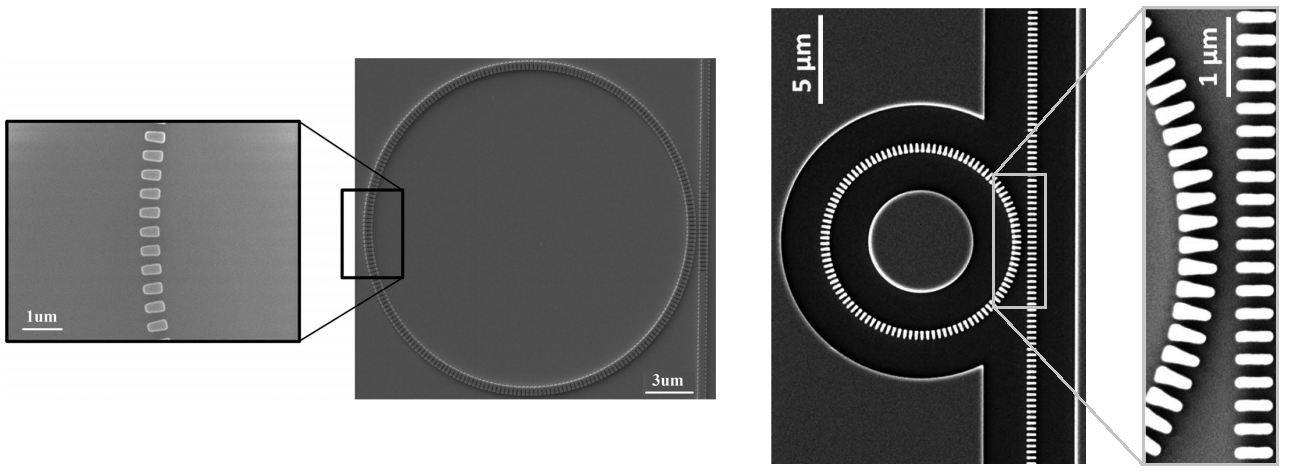
\includegraphics[width=15cm]{SWGSEM.png}
    \caption{\textbf{Left}: From \cite{swg3}. Scanning electron microscope image of one of the first SWG ring resonators used for biosensing. The structure was fabricated using electron beam lithography and is shown in air cladding. Segments have a grating period of 250 nm, duty cycle $\eta$ of 0.7,  an in-plane width of 500 nm, and an out-of-plane thickness of 220 nm.  \\ 
    \textbf{Right:} From  \cite{trapezoidal}. Scanning electron microscope image of a 5 $\mu$m radius T-SWG ORR. The structure was fabricated using electron beam lithography and is shown in air cladding. Segments have a length of 500 nm, long width of 210 nm, short width of 140 nm, and out-of-plane thickness of 250 nm.}
    \label{fig:swgSEM}
\end{figure}

\twocolumngrid

\section{V. Practical Implementations}
\vspace{-1em}

In order to ensure the effectiveness of subwavelength grating micro-ring resonator (SWGMR) devices we must look at how the analytical results compare to the simulated system results, and more importantly how these measure up to the experimental results conducted in the real world. We 

%https://spie.org/news/4131-assessing-silicon-photonic-biosensors-for-home-healthcare?SSO=
\pagebreak


%% add comparison of Q factors, LoDs, Sensitivities, etc. with trapezoidal SWG, regular SWG, conventional strip TE/TM, and **conventional ELISA** LoD.


\section{VI. Conclusion}
\vspace{-1em}
As silicon photonic devices are compatible with existing CMOS foundry processes, ORR biosensors are well-suited for frontline diagnostic applications, such as early detection, drug testing, blood typing, and more.



\bibliographystyle{IEEEtran}
\bibliography{mybib}

\section{Statements of Contribution}
% D.H. 

% S.L.

% Y.L
\vspace{-1em}


\end{document}
